\chapter{T双対性、Dブレーン、ゲージ理論}

\lectureoverview{T双対性は、半径(R)の円上の閉じた弦と\(\alpha'/R\)との間の厳密な等価性として始まる。運動量と巻き数は役割を交換し、世界面の微分\(\partial_\tau Y\)と\(\partial_\sigma Y\)、および\(G_{\mu 5}\)と\(B_{\mu 5}\)から生じる時空ベクトルも同様に交換する。同じ操作を開いた弦に適用すると、ノイマン端点条件がディリクレ条件になる。そのとき端点は動的なDブレーン上になければならない。1枚のブレーンに閉じ込められた開いた弦は低エネルギーでアーベルゲージ理論を生み出す。ブレーンの積み重ねに結合する弦は2つの端点ラベルを持ち、非アーベルゲージ理論を生み出す。D3ブレーン上で終わるD弦は、対応する磁気モノポールを与える。}

\section{なぜT双対性に戻るのか？}

我々はすでにT双対性に出会ったが、理由があってそれに戻る。それは弦理論が摂動的な弦よりもはるかに多くを含むという手がかりの1つであった。開いた弦に対するその帰結が理解されると、それはDブレーンへと導いた。Dブレーンは今度は量子場の理論を構成し研究する方法となった。したがってこの講義の目的は、単に小さな円が大きな円と等価であるというスローガンを繰り返すことではない。そのスローガンがどのようにして新しい物理的対象を理論に強制するかを理解するのに十分注意深く議論を再構築する。

最も単純な設定はトーラス的コンパクト化である。1次元トーラスは円である。2次元トーラスは、対辺が同一視された平行四辺形で表すことができ、3次元トーラスは、対面が同一視された平行六面体で表すことができる。同じ構成はより高い次元でも続く。我々は\(Y\)と呼ばれる1つのコンパクトな空間座標と、\(X\)と呼ばれる1つの代表的な非コンパクト座標のみを保持する。時間は存在するが、板書の図には示されない。

標準的な規約
\begin{equation}
  Y\sim Y+2\pi R,
  \label{eq:l10-circle-identification}
\end{equation}
を選ぶ。すると\(R\)が半径であり、\(2\pi R\)が円周である。講義ではコンパクトな大きさを単に\(r\)と呼び、\(2\pi\)と\(\alpha'\)の因子をしばしば省略する。我々は導出において従来の因子を保持し、有用なときには講義の単位を示す。

議論の前半では、弦は閉じていて向き付けられている。向き付けとは、弦の周りに描かれた内在的な矢印である。至る所ですべての矢印を逆にしても実験は変わらない。重要なのは2つの弦の相対的な向きである。分裂と結合の間、矢印は連続的に結合しなければならない。これは符号付きの保存量が現れるという最初のヒントである。

\begin{figure}[H]
  \centering
  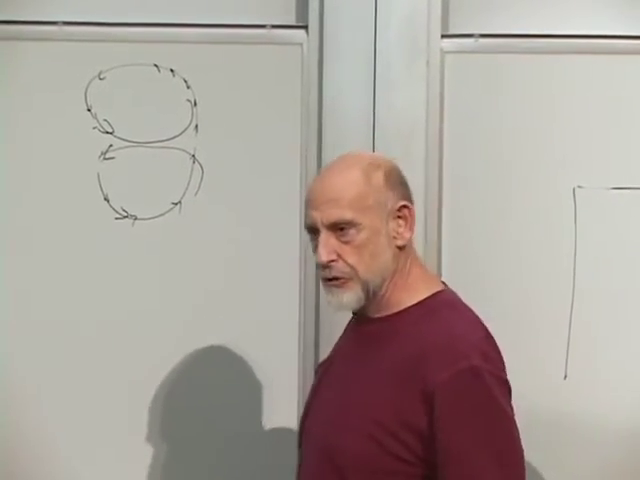
\includegraphics[width=0.72\textwidth]{lecture_10_figure_01.png}
  \caption{相対的な向きが板書に記された2つの閉じた弦。向きは分裂と結合を通じて連続でなければならない。}
  \lectureframe{00:05:40}
  \label{fig:l10-oriented-closed-strings}
\end{figure}

\begin{classroomqa}
\audiencequestion{世界面座標が\(\sigma=0\)から\(2\pi\)まで走るなら、弦はすでにコンパクト方向を一度回ったのか？\lecturetimestamp{00:08:42}}
\lecturerresponse{いいえ。座標\(\sigma\)は弦に沿った点をラベル付けするのであり、コンパクト空間内の位置をラベル付けするのではない。すべての閉じた弦は、巻かれていようと巻かれていなかろうと、周期的なパラメータ\(\sigma\)を持つ。輪ゴムのアナロジーは有用である。輪ゴムが何にも巻き付いていなくても、輪ゴムの周りの分子に番号を付けることができる。巻き数は写像\(Y(\tau,\sigma)\)の性質であり、パラメータ\(\sigma\)だけの性質ではない。}
\end{classroomqa}

\begin{classroomqa}
\audiencequestion{コンパクトな大きさも、大きな座標\(X\)のすべての値で同じでなければならないのか？\lecturetimestamp{00:10:00}}
\lecturerresponse{一般的な動的コンパクト化ではそうではない。我々は最もきれいな背景であるため固定された円から始める。後に成分\(G_{55}\)は、その値が第5方向の局所的な大きさを測るスカラー場になるので、その大きさは通常の時空上で変化し得る。}
\end{classroomqa}

\section{巻き数は弦が再結合しても保存される}

巻かれていない弦は、コンパクト方向を巻き付かずに動くことができる。巻かれた弦は異なる。\(\sigma\)が閉じた弦を一度回るにつれて、埋め込み\(Y(\tau,\sigma)\)はコンパクトな円の1つ以上の周期を進む。弦は向き付けられているので、その進行には符号がある。弦は正の方向に巻くことも、負の方向に巻くこともできる。

保存則は結合の図で最も明瞭である。巻き数\(+1\)の弦と巻き数\(-1\)の弦を取る。それらの適合するセグメントは再結合し得る。結果として得られる配置は正味の巻き数がゼロであり、巻かれていない弦に変形することができる。板書はまさにこの逆向きの再結合をたどる。

\begin{figure}[H]
  \centering
  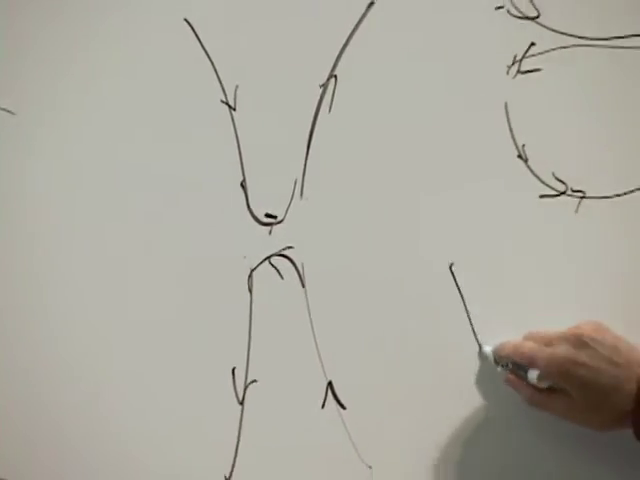
\includegraphics[width=0.72\textwidth]{lecture_10_figure_02.png}
  \medskip

  \begin{tikzpicture}[x=1cm,y=1cm,>=Latex]
    \draw[thick] (-4.0,0.3) circle (0.65);
    \draw[->,thick] (-4.55,0.58) arc (150:-145:0.65);
    \node at (-4.0,-0.65) {$w=+1$};
    \draw[thick] (-2.0,0.3) circle (0.65);
    \draw[<-,thick] (-2.55,0.58) arc (150:-145:0.65);
    \node at (-2.0,-0.65) {$w=-1$};
    \node at (-3.0,0.3) {$+$};
    \draw[->,thick] (-1.0,0.3) -- (0.3,0.3);
    \draw[thick] (1.4,0.3) ellipse (0.95 and 0.55);
    \node at (1.4,-0.65) {$w_{\rm total}=0$};
  \end{tikzpicture}
  \caption{逆向きの巻き付きは再結合して、正味の巻き付きがゼロの
  配置になる。下の図は盤面の操作をきれいに再構成したものであり、
  第二の力学過程ではない。}
  \lectureframe{00:13:20}
  \label{fig:l10-opposite-winding}
\end{figure}

次に、同じ向きをもつ二本の弦で実験を繰り返す。
それらは結合できるが、ほどけることはできない。結果は、入射した
どちらの弦の巻き付きの二倍を担う。結合した弦の本数は変化したが、
全巻き付き数は変化していない。

\begin{figure}[H]
  \centering
  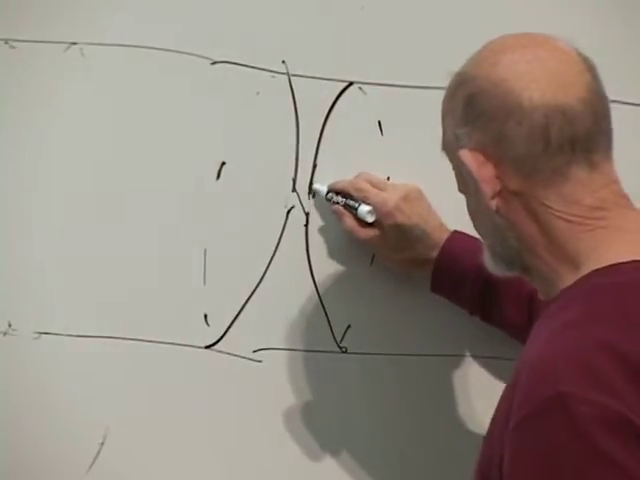
\includegraphics[width=0.72\textwidth]{lecture_10_figure_03.png}
  \medskip

  \begin{tikzpicture}[x=1cm,y=1cm,>=Latex]
    \draw[thick] (-4.0,0.3) circle (0.65);
    \draw[->,thick] (-4.55,0.58) arc (150:-145:0.65);
    \node at (-4.0,-0.65) {$w=+1$};
    \draw[thick] (-2.0,0.3) circle (0.65);
    \draw[->,thick] (-2.55,0.58) arc (150:-145:0.65);
    \node at (-2.0,-0.65) {$w=+1$};
    \node at (-3.0,0.3) {$+$};
    \draw[->,thick] (-1.0,0.3) -- (0.3,0.3);
    \draw[thick] (1.45,0.3) circle (0.78);
    \draw[thick] (1.45,0.3) circle (0.52);
    \draw[->,thick] (0.81,0.74) arc (145:-145:0.78);
    \node at (1.45,-0.78) {$w=+2$};
  \end{tikzpicture}
  \caption{同符号の巻き付きは再結合して二重に巻き付いた弦になりうる。
  連結性は変化するが、全巻き付き数は二のままである。}
  \lectureframe{00:16:40}
  \label{fig:l10-same-winding}
\end{figure}

この区別は許されるあらゆる過程で保たれる。全巻き付き数が百である
状態は、百回巻き付いた一本の弦、それぞれ五十回巻き付いた二本の弦、
あるいは一回ずつ巻き付いた百本の弦によって担われうる。弦はこれらの
記述の間で分裂したり結合したりできるが、符号付きの和は百のままである。
これを\(w\in\mathbb Z\)で表す。

\section{運動量モードと巻き付きモード}

保存則それ自体はまだ双対性ではない。次にエネルギーを比較する。
コンパクトな円の周りを運動する状態は量子化された運動量
\begin{equation}
  p_Y=\frac{n}{R},
  \qquad n\in\mathbb Z.
  \label{eq:l10-compact-momentum}
\end{equation}
をもつ。他の質量への寄与が無視できる状態に対して、コンパクトな
運動は\(E_{\rm mom}=|n|/R\)に寄与する。正と負の\(n\)は反対向きの
運動を表し、エネルギーは正である。

\begin{figure}[H]
  \centering
  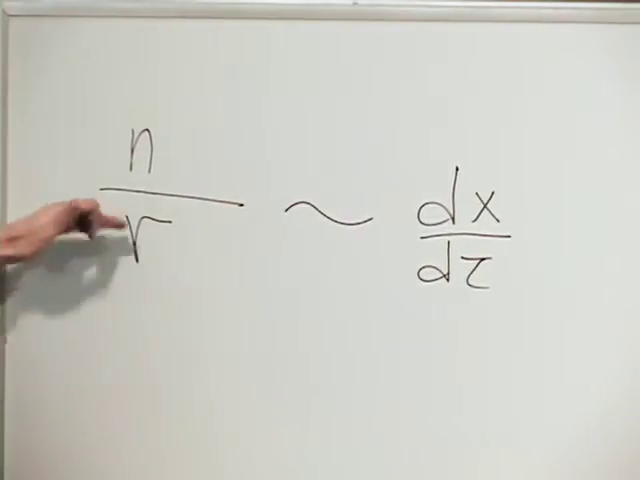
\includegraphics[width=0.72\textwidth]{lecture_10_figure_04.png}
  \caption{盤面上のコンパクトな運動量量子数。講義では運動量を
  コンパクトな速度の積分として模式的に書いている。}
  \lectureframe{00:21:30}
  \label{fig:l10-compact-momentum-board}
\end{figure}

\(|w|\)回巻き付いた弦の長さは\(2\pi |w|R\)である。基本弦の張力
\begin{equation}
  T_{\rm F}=\frac{1}{2\pi\alpha'},
\end{equation}
を用いると、その巻き付きエネルギーは
\begin{equation}
  E_{\rm wind}=T_{\rm F}(2\pi |w|R)
  =\frac{|w|R}{\alpha'}.
  \label{eq:l10-winding-energy}
\end{equation}
である。講義の単位\(\alpha'=1\)では、これは単に\(E_{\rm wind}=|w|R\)である。

二つの塔は半径が変化するにつれて逆の振る舞いをする。\(R\gg
\sqrt{\alpha'}\)では、運動量の準位は間隔が狭く、巻き付きの準位は
間隔が広い。\(R\ll\sqrt{\alpha'}\)では、運動量の準位は間隔が広く、
巻き付きの準位は間隔が狭い。

\begin{figure}[H]
  \centering
  \begin{minipage}[t]{0.48\textwidth}
    \centering
    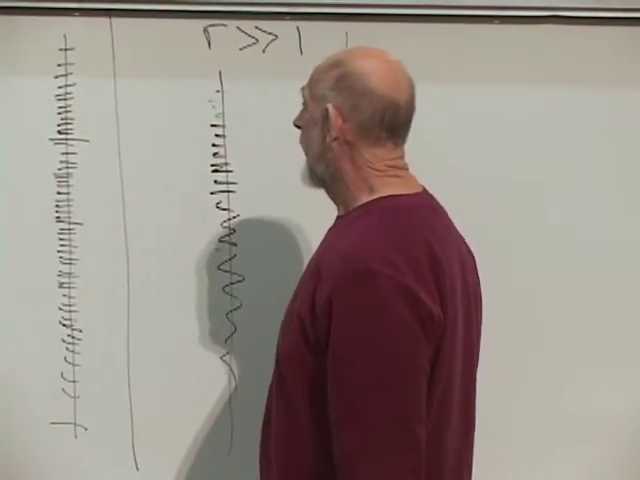
\includegraphics[width=\linewidth]{lecture_10_figure_05.png}
    \par\smallskip
    \textit{大きなコンパクト半径。}
  \end{minipage}\hfill
  \begin{minipage}[t]{0.48\textwidth}
    \centering
    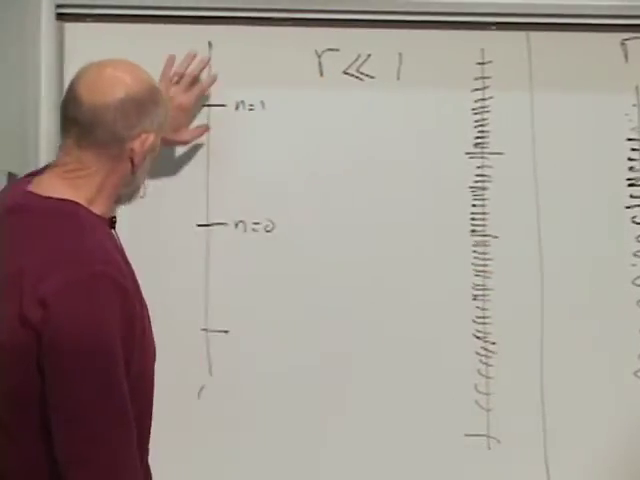
\includegraphics[width=\linewidth]{lecture_10_figure_06.png}
    \par\smallskip
    \textit{小さなコンパクト半径。}
  \end{minipage}
  \caption{盤面上の二つのスペクトルの比較。半径が反転すると、
  疎な塔と密な塔が役割を交換する。}
  \lectureframe{00:25:30--00:26:00}
  \label{fig:l10-dual-spectra-board}
\end{figure}

きれいな模式図は
\begin{figure}[H]
  \centering
  \begin{adjustbox}{max width=\linewidth}
  \begin{tikzpicture}[x=1cm,y=0.74cm,>=Latex]
    \node[font=\bfseries] at (-3.6,6.2) {$R\gg\sqrt{\alpha'}$};
    \draw[->] (-5.1,0) -- (-5.1,5.5) node[above] {$E$};
    \foreach \y in {0.4,1.0,1.6,2.2,2.8,3.4,4.0,4.6}
      \draw (-5.35,\y)--(-4.85,\y);
    \node[align=center] at (-4.25,5.15) {momentum\\dense};
    \draw[->] (-2.2,0) -- (-2.2,5.5) node[above] {$E$};
    \foreach \y in {0.4,2.4,4.4}
      \draw (-2.45,\y)--(-1.95,\y);
    \node[align=center] at (-1.35,5.15) {winding\\sparse};

    \node[font=\bfseries] at (3.6,6.2) {$R\ll\sqrt{\alpha'}$};
    \draw[->] (2.2,0) -- (2.2,5.5) node[above] {$E$};
    \foreach \y in {0.4,2.4,4.4}
      \draw (1.95,\y)--(2.45,\y);
    \node[align=center] at (3.05,5.15) {momentum\\sparse};
    \draw[->] (5.1,0) -- (5.1,5.5) node[above] {$E$};
    \foreach \y in {0.4,1.0,1.6,2.2,2.8,3.4,4.0,4.6}
      \draw (4.85,\y)--(5.35,\y);
    \node[align=center] at (5.95,5.15) {winding\\dense};
  \end{tikzpicture}
  \end{adjustbox}
  \caption{準位間隔の議論の再構成。運動量と巻き付きが
  \(R\leftrightarrow\alpha'/R\)とともに交換されるとき、完全な弦のスペクトルは
  不変である。}
  \label{fig:l10-dual-spectra-redraw}
\end{figure}

観測者がこれらのスペクトルの一方を、それがどのように作られたかを
知らされずに手渡されたとしよう。間隔の狭い塔は大きな円上の運動量
なのか、それとも小さな円上の巻き付きなのか。スペクトルだけでは
言えない。弦理論はさらに強い主張をする。散乱振幅もまた言えない
というのである。二つの記述は
\begin{equation}
  n\longleftrightarrow w,
  \qquad
  R\longleftrightarrow \widetilde R=\frac{\alpha'}{R}.
  \label{eq:l10-radius-duality}
\end{equation}
の下で厳密に等価である。不動点は
\begin{equation}
  R=\sqrt{\alpha'},
  \label{eq:l10-self-dual-radius}
\end{equation}
または講義の単位で\(R=1\)である。その半径では追加の状態が
質量ゼロになりうるので、ゲージ対称性が拡大する。

\begin{classroomqa}
\audiencequestion{巻き付きはスペクトルを書き直すための数学的な便宜に
すぎないのか。\lecturetimestamp{00:27:33}}
\lecturerresponse{いいえ。巻き付きは閉弦ヒルベルト空間の実在の
セクターをラベルし、それらのセクターは相互作用に関与する。
``双対性''という語は、運動量による記述と巻き付きによる記述が
同じ物理の異なる座標であることを意味し、一方のセクターが他方の
ための任意の記憶補助であることを意味しない。}
\end{classroomqa}

\begin{classroomqa}
\audiencequestion{それ自身に写される半径はあるか。
\lecturetimestamp{00:27:58}}
\lecturerresponse{はい。自己双対な値は
\(R=\sqrt{\alpha'}\)であり、盤面で用いられている単位では\(R=1\)である。
二つの塔はそこで出会い、スペクトルは拡大した対称性をもつ。}
\end{classroomqa}

\section{双対性の世界面による形式}

スペクトルによる議論は示唆的であるが、世界面はこの交換をより精密に
する。共形ゲージでは、\(Y\)に共役な運動量は\(\partial_\tau Y\)に
比例する。したがって全コンパクト運動量は
\begin{equation}
  P_Y=\frac{1}{2\pi\alpha'}
      \int_0^{2\pi}d\sigma\,\partial_\tau Y.
  \label{eq:l10-worldsheet-momentum}
\end{equation}
の形をとる。巻き付き数は
\begin{equation}
  w=\frac{1}{2\pi R}
      \int_0^{2\pi}d\sigma\,\partial_\sigma Y
   =\frac{Y(2\pi)-Y(0)}{2\pi R}.
  \label{eq:l10-worldsheet-winding}
\end{equation}

\begin{classroomqa}
\audiencequestion{なぜ閉弦の周りで導関数の積分は消えないのか。\lecturetimestamp{00:32:33}}
\lecturerresponse{なぜなら\(Y\)は周期的な標的空間座標であり、\(\sigma\)-円上の一価実関数ではないからである。世界面の点\(\sigma=2\pi\)は\(\sigma=0\)と同じであるが、被覆直線への埋め込みの持ち上げは\(2\pi wR\)だけ変化する。\(\partial_\sigma Y\)の積分はそのずれを測る。}
\end{classroomqa}

\begin{figure}[H]
  \centering
  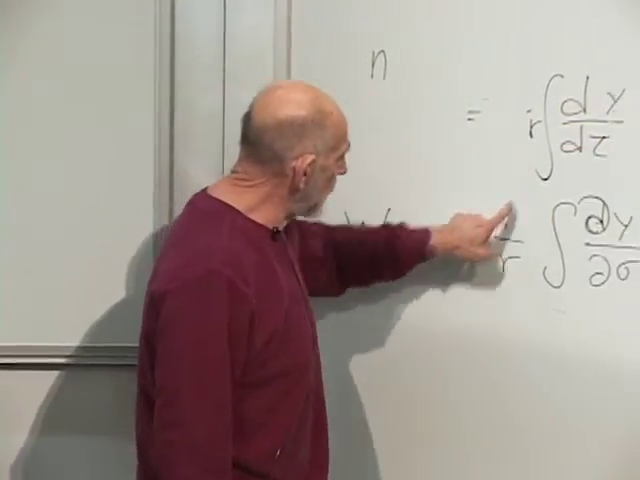
\includegraphics[width=0.76\textwidth]{lecture_10_figure_07.png}
  \caption{両方の線が黒板で完成した後の運動量と巻き付きの積分。共通の\(2\pi\)と\(\alpha'\)の因子は講義の規格化では抑制されている。}
  \lectureframe{00:33:25}
  \label{fig:l10-momentum-winding-integrals}
\end{figure}

一回巻き付いた弦に対して、
\begin{equation}
  Y(\tau,\sigma+2\pi)=Y(\tau,\sigma)+2\pi R.
\end{equation}
巻き付き\(w\)に対して、右辺のずれは\(2\pi wR\)である。式\eqref{eq:l10-worldsheet-winding}はそのとき巻き付きを正確に数える。これが黒板の略記\(w\sim R^{-1}\int
d\sigma\,\partial_\sigma Y\)の正確な版である。

したがってT-双対性の世界面での表現は
\begin{equation}
  \partial_\tau Y\longleftrightarrow
  \partial_\sigma \widetilde Y,
  \qquad
  \partial_\sigma Y\longleftrightarrow
  \partial_\tau \widetilde Y,
  \label{eq:l10-derivative-duality}
\end{equation}
であり、\(Y\)における運動量は双対座標\(\widetilde Y\)における巻き付きになり、その逆も成り立つ。

\begin{classroomqa}
\audiencequestion{これは世界面座標\(\tau\)と\(\sigma\)自体が関係している、あるいは入れ替わっているという意味か。\lecturetimestamp{00:34:39}}
\lecturerresponse{いいえ。T-双対性は解を写し、コンパクトな標的座標の特定の導関数を交換する。それは世界面時間座標を世界面空間座標と同一視するものではない。}
\end{classroomqa}

\section{なぜ巻き付き状態は避けられないのか}

巻き付いていない状態が利用可能であるのに、なぜ弦が巻き付いた状態に見出されることがあるのかと問うかもしれない。弦は好みによってその状態を選ぶのではない。衝突で供給されたエネルギーが弦を引き伸ばす。十分に高エネルギーで高度に歪んだ弦は、反対の巻き付きを持つ二本の弦に再結合しうる。それらの全巻き付きはゼロのままであるが、分裂後、二本の弦は離れうる。対の一方を遠くへ送ることができ、観測者には見かけ上孤立した巻き付き弦が残る。

\begin{figure}[H]
  \centering
  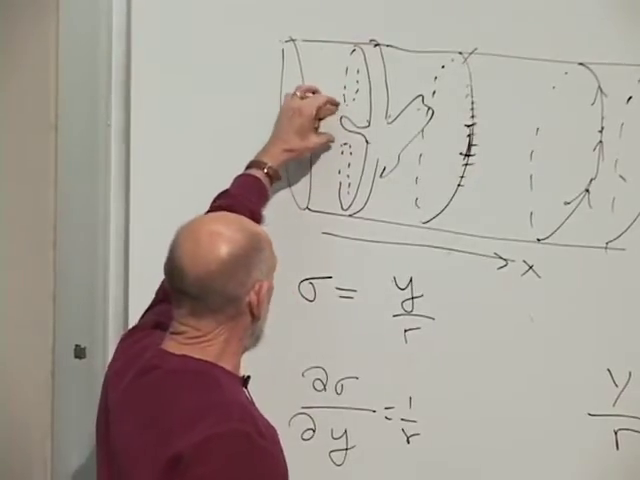
\includegraphics[width=0.76\textwidth]{lecture_10_figure_08.png}
  \caption{再結合後に反対に巻き付いた弦が分離しうる、高度に引き伸ばされた正味巻き付きゼロの配置。}
  \lectureframe{00:36:15}
  \label{fig:l10-winding-pair-production}
\end{figure}

エネルギー閾値は巻き付きエネルギーによって設定される。大きな円では、コンパクト方向の周りに十分な弦を引き伸ばすには大きな衝突エネルギーを要する。しかし閾値以上では、巻き付き--反巻き付き対生成を禁じることはできない。類推は電子--陽電子対を生成する光子衝突である。全電荷は依然としてゼロであるが、荷電粒子は存在し、分離されうる。巻き付きの保存も同じように働く。

この類推は言葉だけのものではない。コンパクト運動量と巻き付きは二つの異なる電荷量子数として振る舞う。対応する還元記述では、同符号は反発し、異符号は引き合う。したがって、それらの力を媒介する二つのベクトル場を問うべきである。

\section{五次元重力からの運動量電荷}

五次元の重力から始める。大文字の添字\(M,N\)は四つの通常の時空方向とコンパクトな第五方向を走るとする。計量は次のように分解される。
\begin{equation}
  G_{MN}\quad\longrightarrow\quad
  \bigl\{G_{\mu\nu},\,G_{\mu5},\,G_{55}\bigr\}.
  \label{eq:l10-metric-decomposition}
\end{equation}
対称成分\(G_{5\mu}\)は\(G_{\mu5}\)を超える新しい情報を含まない。

\begin{figure}[H]
  \centering
  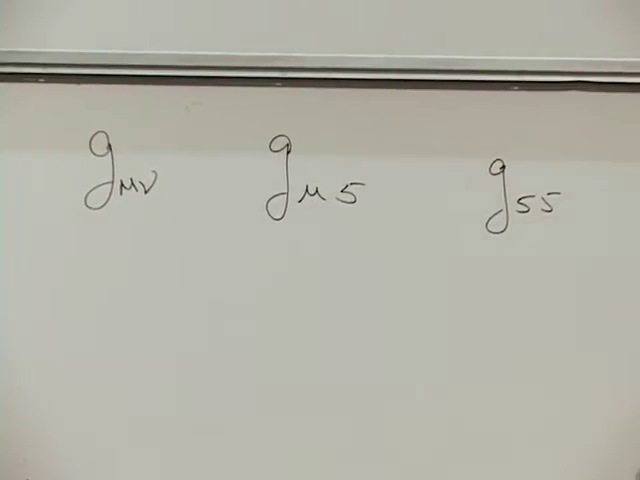
\includegraphics[width=0.74\textwidth]{lecture_10_figure_09.png}
  \caption{五次元計量成分の独立な群：\(G_{\mu\nu}\)、\(G_{\mu5}\)、\(G_{55}\)。}
  \lectureframe{00:44:05}
  \label{fig:l10-metric-components}
\end{figure}

四次元の観点からは、
\begin{align}
  G_{\mu\nu} &\quad\hbox{is a spacetime metric},\\
  G_{\mu5} &\equiv A_\mu\quad\hbox{is a vector field},\\
  G_{55} &\equiv e^{2\varphi}\quad\hbox{is a scalar modulus}.
  \label{eq:l10-four-dimensional-fields}
\end{align}
スカラー\(\varphi\)はコンパクト方向の大きさを測る。それは通常の時空上で滑らかに変動しうるので、\(\varphi\)の波は第五次元の半径の波である。

\begin{figure}[H]
  \centering
  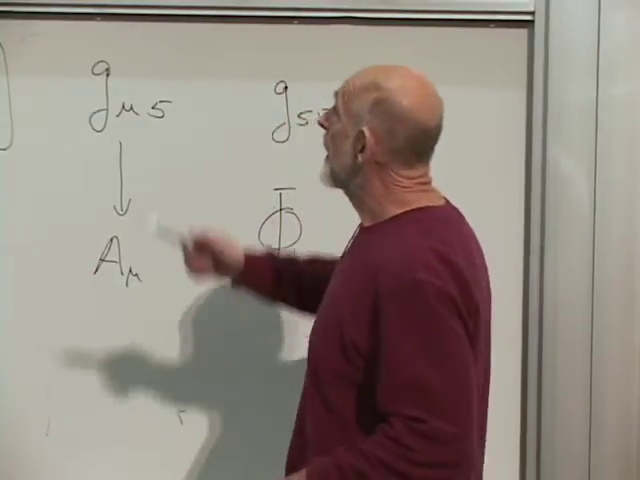
\includegraphics[width=0.74\textwidth]{lecture_10_figure_10.png}
  \caption{黒板は\(G_{\mu5}\)をベクトル\(A_\mu\)と同一視し、\(G_{55}\)をスカラー\(\Phi\)と同一視する。}
  \lectureframe{00:47:40}
  \label{fig:l10-vector-and-radius-modulus}
\end{figure}

混合重力成分の源は混合運動量流である。特に、第五方向の周りの運動量が\(G_{\mu5}\)を源とする。したがって四次元の観測者は整数\(n\)を\(A_\mu\)に結合した電荷と解釈する。これがKaluza--Klein機構である：高次元幾何学における運動量が、低次元場の理論における電荷になる。

\editorialnote{講義は\(G_{55}\)からのスカラーを``ディラトン''と大まかに呼んでいる。この還元ではそれは具体的には半径モジュラスである。弦結合を制御する十次元弦ディラトンは別の場であるが、低次元のスカラー結合は枠と双対性の変化の下で混合しうる。}

\begin{classroomqa}
\audiencequestion{スカラー\(\varphi\)は運動量の整数\(n\)に比例するか？\lecturetimestamp{00:48:43}}
\lecturerresponse{いいえ。整数\(n\)は量子化された状態をラベル付けし、電荷として働く。スカラー\(\varphi(x)\)は連続場であり、局所的なコンパクト化の大きさを決定する。それは場所ごとに変化しうるが、それ自体は整数ではない。}
\end{classroomqa}

\section{第2のベクトル場と巻き付き電荷}

巻き付きもまた電荷のようなものであるが、同じベクトルに同じ仕方で結合することはできない。第2のベクトルを見るために、最初の閉弦励起に戻ろう。閉弦は左向きと右向きの振動子モードをもつ。物理的状態はレベルマッチングを満たす。すなわち、左向きと右向きの全励起レベルが一致しなければならない。

ボソン的理論では、無励起状態はタキオンである。左向きまたは右向きの振動子が1つだけではレベルマッチングを破る。したがって、最初に許される質量ゼロ状態は各種類の振動子を1つずつ含む。
\begin{equation}
  \alpha_{-1}^{I}\widetilde\alpha_{-1}^{J}\ket{0;k}.
  \label{eq:l10-first-massless-state}
\end{equation}
添字\(I,J\)は、コンパクト方向を含む横方向の空間方向にわたって走る。一方の添字が通常の方向で他方が\(5\)であれば、2つのベクトル的振動子状態がある。
\begin{equation}
  \alpha_{-1}^{\mu}\widetilde\alpha_{-1}^{5}\ket{0;k},
  \qquad
  \alpha_{-1}^{5}\widetilde\alpha_{-1}^{\mu}\ket{0;k}.
  \label{eq:l10-two-vector-states}
\end{equation}

\begin{figure}[H]
  \centering
  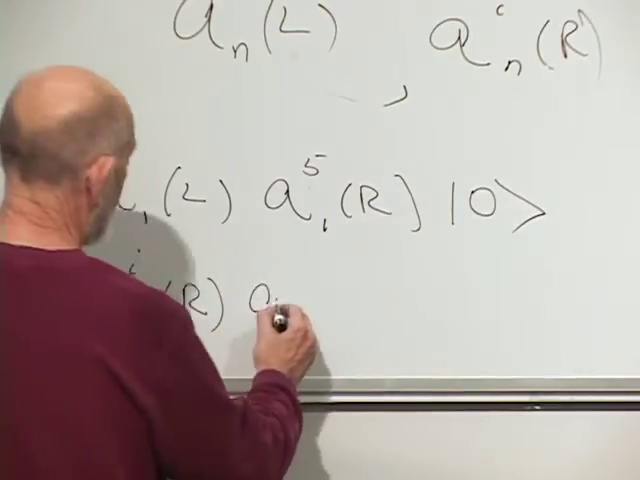
\includegraphics[width=0.76\textwidth]{lecture_10_figure_11.png}
  \caption{一方の偏極がコンパクト方向に沿っているときに4次元ベクトル状態となる、2つの左--右振動子の順序。}
  \lectureframe{00:58:20}
  \label{fig:l10-two-vector-states-board}
\end{figure}

それらの対称および反対称の組み合わせは、異なる時空場に属する。
\begin{align}
  \alpha_{-1}^{(\mu}\widetilde\alpha_{-1}^{5)}\ket{0;k}
    &\longleftrightarrow G_{\mu5},\\
  \alpha_{-1}^{[\mu}\widetilde\alpha_{-1}^{5]}\ket{0;k}
    &\longleftrightarrow B_{\mu5}.
  \label{eq:l10-g-and-b-vectors}
\end{align}
第1のものはコンパクト運動量を源とするKaluza--Kleinベクトルである。第2のものは反対称Kalb--Ramond場に由来し、弦の巻き付きを源とする。したがって、次元還元された理論は2つの光子様場を含み、それぞれが各電荷セクターに対応する。

両方の振動子添字がコンパクト方向に沿っているなら、その状態はコンパクト化のモジュラスに関連するスカラーである。両方が通常の横方向にあるなら、対称トレースレス部分はグラビトンであり、反対称部分は\(B_{\mu\nu}\)であり、トレースはスカラーセクターに寄与する。

\begin{classroomqa}
\audiencequestion{これらの状態のうちどれが一重項でどれが三重項か？\lecturetimestamp{01:00:21}}
\lecturerresponse{その分類はここでは有用ではない。両方の混合状態は4次元ベクトルとして変換する。それらの和と差は、対称な計量偏極と反対称な\(B\)場偏極を分離する。2つのコンパクト添字をもつ状態は代わりに4次元スカラーである。}
\end{classroomqa}

休憩前に到達した完全な対応表は
\begin{equation}
  \boxed{
  \begin{gathered}
    n\leftrightarrow w,
    \qquad
    R\leftrightarrow\dfrac{\alpha'}{R},\\
    \partial_\tau Y\leftrightarrow\partial_\sigma\widetilde Y,
    \qquad
    G_{\mu5}\leftrightarrow B_{\mu5}.
  \end{gathered}}
  \label{eq:l10-complete-t-duality-map}
\end{equation}

\begin{figure}[H]
  \centering
  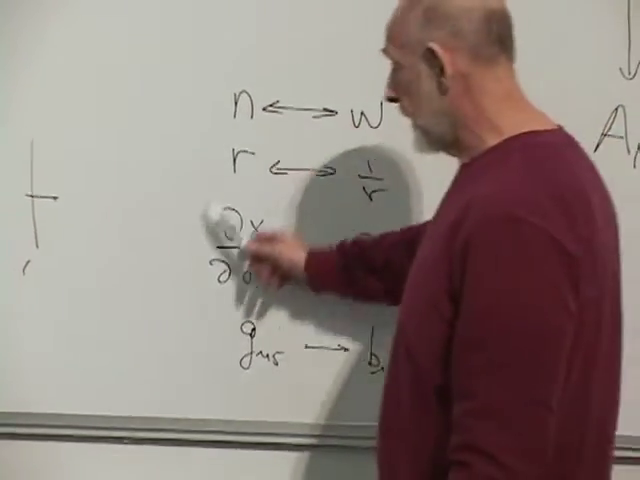
\includegraphics[width=0.72\textwidth]{lecture_10_figure_12.png}
  \caption{T双対性写像の板書要約：運動量と巻き付き、半径と逆半径、世界面微分、および2つのベクトル場が交換される。講師は最終行を一部隠しているため、それは式
  \eqref{eq:l10-complete-t-duality-map}
  に明示的に与えられている。}
  \lectureframe{01:02:20}
  \label{fig:l10-t-duality-map-board}
\end{figure}

この構成は、今列挙したすべての場がすでに観測された粒子スペクトル中で同定されたという主張と混同されるべきではない。この時点では、それはコンパクト化された弦理論の数学的帰結である。そのような構造を現象論に結びつける提案は数多くあるが、それはこの講義で解かれている問題ではない。

\section{開弦は問いを変える}

休憩後、開弦から再び始める。閉弦は安定な巻き付きをもちうる。なぜなら、巻き付きが逃げ出す端点をもたないからである。開弦は端点をもつため、同様の位相的に保護された巻き付き数をもたない。それでもT双対性は理論の厳密な対称性である。この対称性は開弦に何をするのか？

自由に動く端点に対して、弦の作用の変分はNeumann境界条件を与える。単純な\((X,Y)\)幾何では、
\begin{equation}
  \left.\partial_\sigma X\right|_{\partial\Sigma}=0,
  \qquad
  \left.\partial_\sigma Y\right|_{\partial\Sigma}=0.
  \label{eq:l10-neumann-boundary}
\end{equation}
力学的描像は単純である。弦をますます小さな質量要素の連鎖とみなす。最後の要素に非ゼロの接線方向の力が働けば、その質量がゼロに近づくにつれて発散する加速度を与えることになる。したがって自由な端点は、端点張力の正味が消えるまで調整する。代わりに端点を固定し、必要な力を与えることもできるが、その場合端点はもはや自由ではない。

\begin{figure}[H]
  \centering
  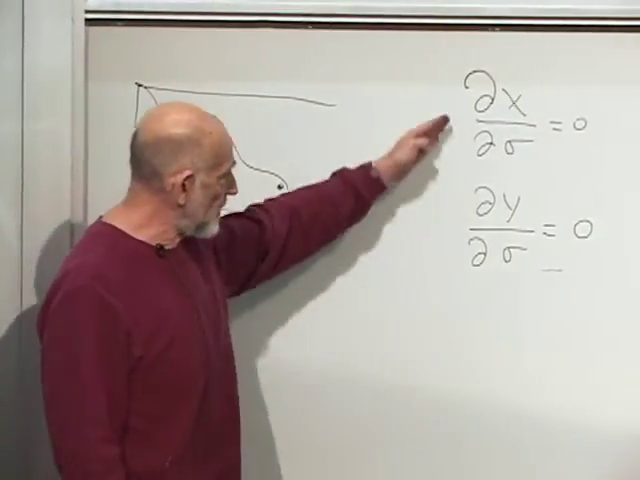
\includegraphics[width=0.76\textwidth]{lecture_10_figure_13.png}
  \caption{開弦とその完成されたNeumann端点条件、
  \(\partial_\sigma X=\partial_\sigma Y=0\)。}
  \lectureframe{01:09:20}
  \label{fig:l10-neumann-board}
\end{figure}

ここで、コンパクト座標\(Y\)のみを双対化する。非コンパクト座標\(X\)は変わらない。式\eqref{eq:l10-derivative-duality}により、第二のノイマン条件は
\begin{equation}
  \left.\partial_\tau\widetilde Y\right|_{\partial\Sigma}=0.
  \label{eq:l10-dirichlet-time-derivative}
\end{equation}
となる。したがって、端点は双対化されたコンパクト方向において時間に依存しない位置をもつ：
\begin{equation}
  \left.\widetilde Y\right|_{\partial\Sigma}=Y_0.
  \label{eq:l10-dirichlet-boundary}
\end{equation}
これがディリクレ境界条件である。

\begin{figure}[H]
  \centering
  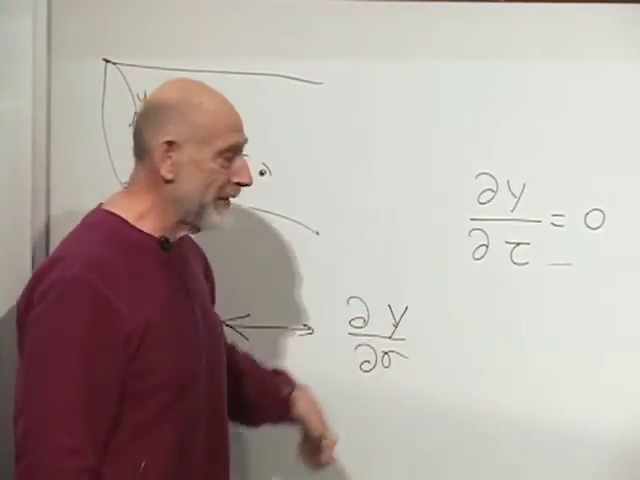
\includegraphics[width=0.76\textwidth]{lecture_10_figure_14.png}
  \medskip

  \begin{adjustbox}{max width=\linewidth}
  \begin{tikzpicture}[x=1cm,y=1cm,>=Latex]
    \node[align=center] at (-3.5,0.8)
      {Neumann\\\(\left.\partial_\sigma Y\right|_{\partial\Sigma}=0\)};
    \draw[->,thick] (-1.7,0.8) -- (1.3,0.8)
      node[midway,above] {$T_Y$};
    \node[align=center] at (3.4,0.8)
      {Dirichlet\\\(\left.\partial_\tau\widetilde Y\right|_{\partial\Sigma}=0\)};
    \node[align=center] at (3.4,-0.5)
      {\(\widetilde Y(\tau)=Y_0\) at each endpoint};
  \end{tikzpicture}
  \end{adjustbox}
  \caption{黒板に完成した双対端点条件と、その明快な論理的再構成。T双対性は、コンパクト方向の自由度を、双対方向における固定された端点位置に変える。}
  \lectureframe{01:12:35}
  \label{fig:l10-neumann-to-dirichlet}
\end{figure}

\begin{classroomqa}
\audiencequestion{なぜ双対条件は端点が固定されていることを意味するのか。\lecturetimestamp{01:12:39}}
\lecturerresponse{なぜなら\(\partial_\tau\widetilde Y=0\)は双対化された方向における速度ゼロだからである。端点が\(\widetilde Y\)のどこから始まっても、そこにとどまる。双対化されていない方向に平行な座標は依然として自由である。}
\end{classroomqa}

\section{端点を保持する対象はDブレーンである}

端点が固定されているなら、それをそこに保持できる何かが存在しなければならない。したがって、厳密なT双対性は、開弦が端を置ける新しい対象を必要とする。その対象がDブレーンである。文字\(D\)はディリクレを表し、対象の次元を表すのではない。講義の歴史的余談では、その力学的役割を疑いようのないものにしたジョセフ・ポルチンスキーにちなんでこれらの対象が名づけられたかもしれないが、すでに定着していた用語``pブレーン''のため、ディリクレが自然な名称として残った。

\(p\)ブレーンは\(p\)個の空間次元をもつ。弦は1ブレーン、膜は2ブレーン、拡がった三次元物体は3ブレーンである。D\(p\)ブレーンは\(p\)ブレーンであり、その上では基本弦の端点が横方向にディリクレ条件を、ブレーンに接する方向にノイマン条件を満たす。

双対性の議論のどこにも\(Y_0\)のある特定の値を選び出すものはないので、Dブレーンは宇宙の特定の点に釘付けにされた剛体の固定物ではありえない。それは可動でなければならない。相対性理論も絶対的に剛体な拡がった物体を禁じるので、Dブレーンは揺らぎ、曲がることができる。黒板に描かれた単純な平坦ブレーンはその平衡配置であり、その力学を制限するものではない。

\begin{classroomqa}
\audiencequestion{開弦の二つの端点は、双対座標の同じ固定値をもたなければならないのか。\lecturetimestamp{01:14:55}}
\lecturerresponse{一般にはそうではない。両端点は同じDブレーン上にあり、その場合にはそのブレーンの横方向の位置を共有する。また、異なる横方向位置にある二つの異なるDブレーン上にあってもよく、その場合弦はそれらの間に張られる。ブレーン自体が揺らぎ、曲がりうるので、端点の軌跡は完全に平坦な平面にとどまる必要はない。}
\end{classroomqa}

\section{Dブレーンの次元を数える}

十次元超弦理論には九つの空間次元がある。T双対性が一つの空間方向にディリクレ条件を課すとしよう。端点は他の八方向では依然として自由なので、その許される軌跡は八次元D8ブレーンである。追加の独立なディリクレ条件はそれぞれ、端点の運動の一方向を除く。\(k\)個の空間座標が固定されるなら、
\begin{equation}
  p=9-k.
  \label{eq:l10-dp-counting}
\end{equation}

卓上は同じ数え方の三次元版を与える。鉛直座標を固定すれば、指先は二次元の卓上を動ける。第二の座標を固定すれば、それはもはや線に沿ってのみ動ける。三つすべてを固定すれば、それは一点に閉じ込められる。

\begin{figure}[H]
  \centering
  \begin{adjustbox}{max width=\linewidth}
  \begin{tikzpicture}[x=1.05cm,y=1cm,>=Latex]
    \draw[fill=blue!8] (-5.5,-0.7) -- (-2.5,-0.7) -- (-1.7,0.2)
      -- (-4.7,0.2) -- cycle;
    \node at (-3.6,-1.15) {one constraint: sheet};
    \draw[very thick,blue!60!black] (-0.9,-0.25) -- (1.3,-0.25);
    \node at (0.2,-1.15) {two constraints: line};
    \fill[blue!70!black] (4.1,-0.25) circle (0.09);
    \node at (4.1,-1.15) {three constraints: point};
    \draw[->] (-1.45,0.95) -- (-0.75,0.95);
    \draw[->] (2.25,0.95) -- (2.95,0.95);
    \node at (0.35,1.35) {each Dirichlet condition lowers \(p\) by one};
  \end{tikzpicture}
  \end{adjustbox}
  \caption{卓上で用いられた次元の数え上げの議論。D\(p\)ブレーンは、端点が自由に動ける軌跡である。}
  \label{fig:l10-dp-counting-redraw}
\end{figure}

双対性を繰り返すと、D8、D7、D6ブレーンなどが生成され、D0ブレーンに至る。後者は空間的に点状である。空間方向が固定されなければ、D9ブレーンは九つの空間次元すべてを満たし、通常の開弦はどこへでも自由に動ける。講義ではD\((-1)\)ブレーンに簡単に触れている。これらはユークリッド時空に局在し、時間を通って伝播する通常の粒子としてではなく、インスタントンとして振る舞う。

\editorialnote{次元の梯子は、タイプII理論をまとめて扱った場合についての主張である。安定なBPS D\(p\)ブレーンは、タイプIIAでは偶数\(p\)を、タイプIIBでは奇数\(p\)をもつ。一つの円に沿ったT双対性は\(p\)を1だけ変え、同時にタイプIIAとタイプIIBを交換する。}

\begin{classroomqa}
\audiencequestion{もし6次元だけがコンパクトなら、数え上げは9ではなく6から引くことから始めるべきではないか？ \lecturetimestamp{01:20:49}}
\lecturerresponse{初等的な導出ではコンパクト方向にT双対性を施すが、双対な円は元の円が任意に小さくなるにつれて任意に大きくなる。その極限では実質的に非コンパクトである。したがって得られるブレーンは、到達可能なスケールでは非コンパクトに見える方向に沿って伸びることも、それに横たわることもできる。次元\(p\)はブレーンに接するすべての空間方向を数えており、ある一つの導出で用いたコンパクトな方向だけを数えているのではない。}
\end{classroomqa}

D0ブレーンは新しい種類の粒子である。開弦は一つのD0ブレーンから別のブレーンへ走り、同じD0ブレーンに戻ることも、非常に遠く離れたブレーンに向かって伸びることもできる。文字通り空間的無限遠まで伸びた弦は無限の長さを持ち、したがって無限のエネルギーを持つので、物理的に有用な版ではもう一方の端点を別の物体の上に置く。

次の場合であるD1ブレーンは、それ自体が弦の形をしているが、我々が出発点とした基本弦ではない。それは曲がったり自分自身で閉じたりでき、基本弦はその上で終わることができる。その張力は弦結合定数に対して異なるスケーリングをする：
\begin{equation}
  T_{\rm D1}=\frac{1}{2\pi\alpha' g_s},
  \qquad
  T_{\rm F1}=\frac{1}{2\pi\alpha'}.
  \label{eq:l10-dstring-tension}
\end{equation}
弱結合\(g_s\ll1\)では、D弦は基本弦よりずっと重く、このことがそれが最初に重い錨として現れる理由を説明する。

\begin{figure}[H]
  \centering
  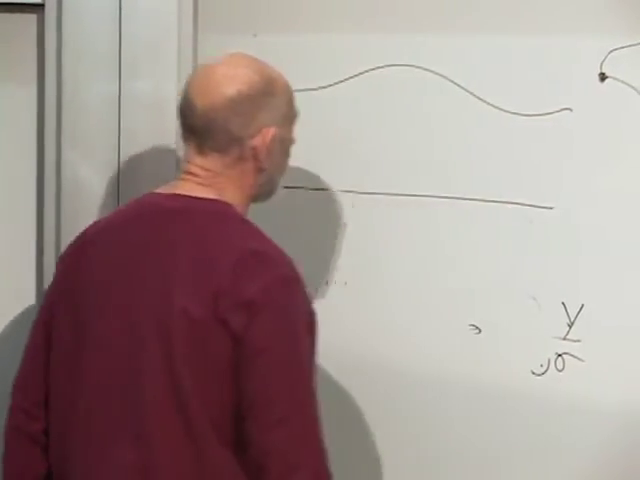
\includegraphics[width=0.76\textwidth]{lecture_10_figure_15.png}
  \caption{板書のD1ブレーン：曲がり得る1次元の物体であり、その上で終わり得る基本弦とは別物である。}
  \lectureframe{01:24:20}
  \label{fig:l10-d1-brane}
\end{figure}

\begin{classroomqa}
\audiencequestion{T双対性は弦だけでなくDブレーンにも作用するのか？ \lecturetimestamp{01:25:35}}
\lecturerresponse{はい。D\(p\)ブレーンに平行なT双対性はその次元をD\((p-1)\)に下げ、それに横たわるT双対性は次元をD\((p+1)\)に上げる。ブレーンは双対性の辞書の一部であり、それによって変わらずに残される外部の支えではない。}
\end{classroomqa}

\begin{classroomqa}
\audiencequestion{ブレーンに接する方向は依然としてコンパクトであり得るか？
\lecturetimestamp{01:27:25}}
\lecturerresponse{はい。``接する''ということと``コンパクト''であることは異なる問いに答える。ある方向はブレーンに沿っていながら円に閉じることもでき、また非コンパクトであることもできる。端点にとって重要なのは、その方向の境界条件がノイマンかディリクレかである。}
\end{classroomqa}

D2ブレーンは膜のようなシートである。D3ブレーンは3つの空間次元を持つ。真に高次元の時空では、D3ブレーンは空間全体ではなく3次元部分空間である。たとえそこに閉じ込められた観測者にとってはそれが空間世界の全体として経験されるとしても。

\begin{figure}[H]
  \centering
  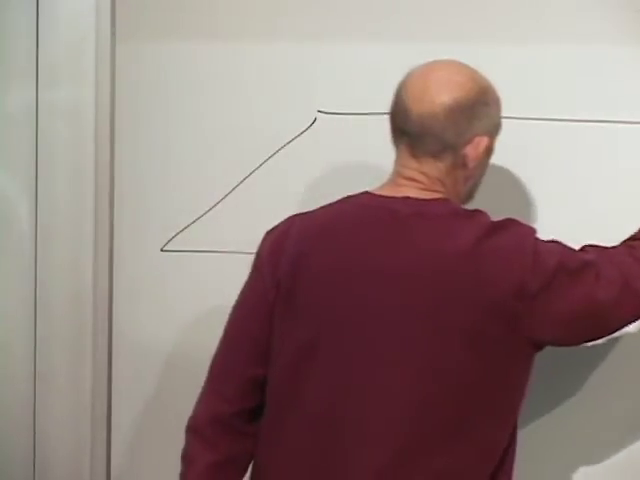
\includegraphics[width=0.76\textwidth]{lecture_10_figure_16.png}
  \caption{弦の端点が動けるシートとして描かれたD2ブレーン。}
  \lectureframe{01:27:55}
  \label{fig:l10-d2-brane}
\end{figure}

ここで与えた導出は意図的に概略である。それ自体は弦理論が自然を記述する証明ではない。しかし弦理論の内部では、整合性の検査は数多い：双対性、量子計算、数学的結果のすべてが、Dブレーンが真の力学的物体であることを指し示している。

\section{開いた弦はブレーン上の場になる}

それ以外は空のD2ブレーンを取り、その上に短い開いた弦を置く。各端点はシートに閉じ込められているので、低エネルギー励起全体はシートに沿って動く。隣接する端点が整合する矢印を持つ2本の有向弦は結合できる。結合した弦は後に再び分裂してもよい。粒子の履歴として読めば、これらはファインマン図の頂点である：2つの粒子が入り、中間励起が伝播し、2つの粒子が出る。

\begin{figure}[H]
  \centering
  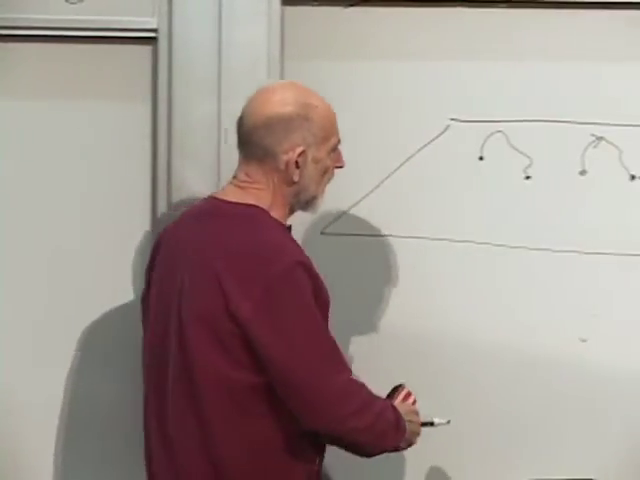
\includegraphics[width=0.76\textwidth]{lecture_10_figure_17.png}
  \caption{D2ブレーン上の有向開弦が整合する端点を通じて結合する。低エネルギーでは、この過程はブレーン上の場の理論の相互作用として読まれる。}
  \lectureframe{01:29:55}
  \label{fig:l10-open-strings-on-brane}
\end{figure}

弦スケールより十分低いエネルギーでは、内部の振動の塔は励起されない。残る質量ゼロの開弦状態はブレーンの世界体積上のベクトル場である。1枚のブレーンに対してこれはアーベル\(U(1)\)ゲージ場であり、電磁気学のブレーン版である。この場は10次元のバルク全体を伝播せず、その量子は端点によってブレーン上に保たれる開弦である。

\section{ブレーンの積み重ねは非アーベル色を生む}

ここで、いくつかの平行なブレーンを互いに近くに置く。3枚のブレーンについては、それらを赤、緑、青とラベル付けする。向き付けられた弦は、端点ラベルの順序対をもつ。すなわち、赤から緑へ、緑から青へ、赤から赤へ、などと走ることができる。\(N\)枚のブレーンでは、質量のない開弦状態は\(N\times N\)行列として並べることができる。
\begin{equation}
  A_\mu{}^{i}{}_{j},
  \qquad i,j=1,\ldots,N.
  \label{eq:l10-chan-paton-matrix}
\end{equation}
これらは\(U(N)\)ゲージ理論のChan--Patonラベルである。

\begin{figure}[H]
  \centering
  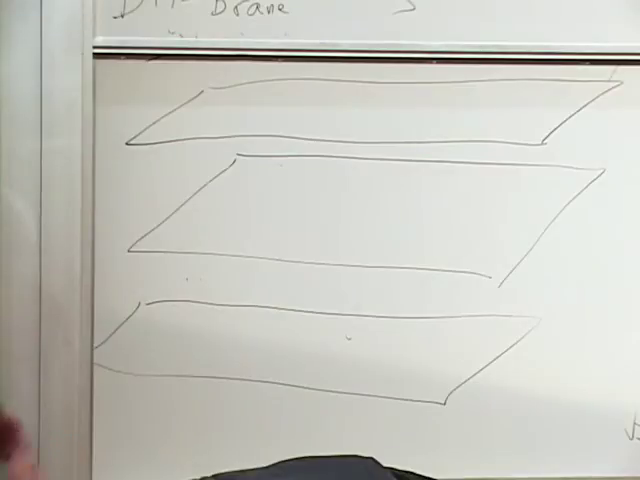
\includegraphics[width=0.76\textwidth]{lecture_10_figure_18.png}
  \medskip

  \begin{adjustbox}{max width=\linewidth}
  \begin{tikzpicture}[x=1cm,y=1cm,>=Latex]
    \draw[very thick,red!70!black] (-4.8,2.0)--(4.8,2.0);
    \draw[very thick,green!55!black] (-4.8,0.8)--(4.8,0.8);
    \draw[very thick,blue!70!black] (-4.8,-0.4)--(4.8,-0.4);
    \node[left] at (-4.8,2.0) {Red};
    \node[left] at (-4.8,0.8) {Green};
    \node[left] at (-4.8,-0.4) {Blue};
    \draw[->,thick] (-3.4,2.0) .. controls (-2.8,1.35) and (-2.3,1.15)
      .. (-1.7,0.8);
    \node at (-2.7,1.05) {$R\!G$};
    \draw[->,thick] (-0.6,0.8) .. controls (0.0,0.25) and (0.6,-0.05)
      .. (1.2,-0.4);
    \node at (0.1,0.0) {$G\!B$};
    \draw[->,thick] (2.1,2.0) .. controls (2.9,2.55) and (3.8,2.55)
      .. (4.3,2.0);
    \node at (3.2,2.65) {$R\!R$};
  \end{tikzpicture}
  \end{adjustbox}
  \caption{黒板上の3枚の平行なブレーンと、それらの間の弦が担う順序付けられた端点ラベルの明快な再構成。}
  \lectureframe{01:33:15}
  \label{fig:l10-three-brane-stack}
\end{figure}

\begin{classroomqa}
\audiencequestion{弦は、他の描画に遮られることなく、本当に赤ブレーンから緑ブレーンへ走ることができるのか。\lecturetimestamp{01:35:07}}
\lecturerresponse{はい。ブレーンはより高次元の空間に埋め込まれている。2次元の黒板の絵は射影にすぎないので、弦は別の射影された線の周りを横断方向に回り込んで通ることができる。}
\end{classroomqa}

\begin{classroomqa}
\audiencequestion{赤--緑弦は、赤--青弦になるために緑--青弦と結合しなければならないのか。\lecturetimestamp{01:35:39}}
\lecturerresponse{それが基本的な局所的結合規則である。適合する端点どうしが出会い、2つの断片は1本の弦になり、結合されなかった端点は赤と青のラベルを保つ。より複雑な過程は、同じ操作を繰り返すことによって組み立てられる。}
\end{classroomqa}

結合規則は、行列積を幾何学的にしたものである。赤--緑弦は緑--青弦と結合できる。一方の緑端点が他方の緑端点と適合するからである。結果は赤--青弦である。
\begin{equation}
  (R,G)\circ(G,B)\longrightarrow(R,B).
  \label{eq:l10-color-composition}
\end{equation}
繰り返された添字は結合され、内部的に消える。これはYang--Mills相互作用頂点に現れるのと同じ添字構造である。

\begin{figure}[H]
  \centering
  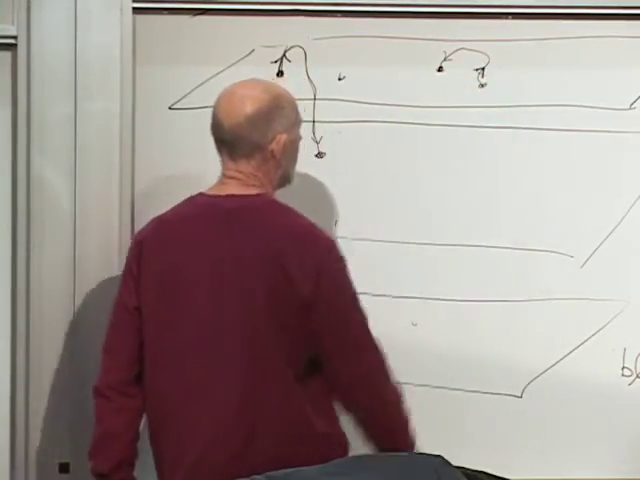
\includegraphics[width=0.76\textwidth]{lecture_10_figure_19.png}
  \caption{スタック上の開弦の結合。端点の向きが、非可換ゲージ場で用いられるのと同じ順序付き添字の合成を強制する。}
  \lectureframe{01:36:30}
  \label{fig:l10-color-joining-board}
\end{figure}

3枚の一致したブレーンに対して、完全な開弦ゲージ群は\(U(3)\)であり、9個のベクトル状態をもつ。その代数は次のように分解される。
\begin{equation}
  \mathfrak u(3)=\mathfrak{su}(3)\oplus\mathfrak u(1).
  \label{eq:l10-u3-decomposition}
\end{equation}
8個のトレースレスな組み合わせはQCDグルーオンの色構造をもつが、対角な重心\(U(1)\)は別個の可換場である。

\editorialnote{講義では、9個の色対の組み合わせのうちの1つが切り離されて消えることができ、それによって8個のグルーオンが残ると説明している。Dブレーンについての正確な記述は、3枚の一致したブレーンのスタックが\(SU(3)\)だけでなく\(U(3)\)を与えるというものである。QCDの八重項を得るには、対角な\(U(1)\)を分離するか、射影で除くか、あるいは他の方法で切り離す必要がある。講義の描像は順序付き色添字を正しく動機づけるが、QCDの完全な導出ではない。}

クォーク様の物質は1つの色添字だけをもつ。ブレーン描像では、それは一方の端点が色スタック上にあり、他方の端点が異なる遠方のブレーン上にある弦によって表される。色スタックに対しては、一方の端だけが色ラベルとして見える。向きを逆にすると反粒子が得られる。適合する端点をもつクォーク様弦と反クォーク様弦は結合して色スタックを離れることができるが、同じ向きの2本のクォーク様弦はそのようには対消滅できない。

得られる低エネルギー理論は一般に超対称Yang--Mills理論であり、追加の物質はブレーンとその交差によって決まる。それらはQCDに十分近く、非可換ダイナミクスを照らし出すが、自動的に標準模型になるわけではない。ブレーンが1枚だけの場合、同じ構成は\(U(1)\)理論に帰着する。短いブレーン--ブレーン弦は光子様であり、第2のセクターに達する向き付けられた弦は正と負の電荷の役割を果たす。

\section{D弦は磁気単極子として終わる}

ここで、物語には2種類の弦様の対象がある。元々の基本弦、すなわちF弦は、D3ブレーン上の電束を担う。D1ブレーン、すなわちD弦は、弱結合でははるかに重い。D弦もD3ブレーン上で終わることができる。その端点はワールドボリュームのゲージ場に対して電気的に荷電しているのではなく、磁気的に荷電している。D3ブレーン上の観測者から見ると、その端点は磁気単極子である。

\begin{figure}[H]
  \centering
  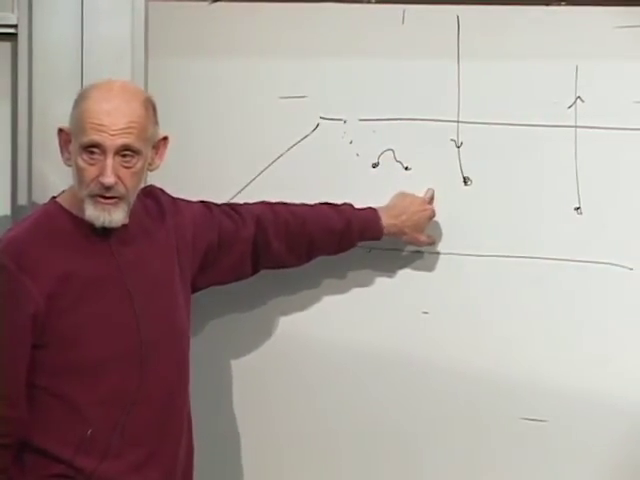
\includegraphics[width=0.76\textwidth]{lecture_10_figure_20.png}
  \medskip

  \begin{adjustbox}{max width=\linewidth}
  \begin{tikzpicture}[x=1cm,y=1cm,>=Latex]
    \draw[fill=blue!7] (-3.8,-0.5)--(2.6,-0.5)--(3.6,0.35)--(-2.8,0.35)--cycle;
    \node at (2.25,-0.95) {D3-brane};
    \draw[very thick,red!70!black] (0.0,3.0)--(0.0,0.0);
    \fill[black] (0.0,0.0) circle (0.08);
    \node[right] at (0.15,2.1) {D-string};
    \foreach \a in {25,65,115,155} {
      \draw[->,blue!65!black] (0.0,0.0)--({1.25*cos(\a)},{0.65*sin(\a)});
    }
    \node[align=center] at (4.8,1.7) {magnetic flux\\on the D3 worldvolume};
    \draw[->] (3.7,1.35)--(1.05,0.45);
  \end{tikzpicture}
  \end{adjustbox}
  \caption{黒板上の端点構成とその明快な解釈。D3ブレーン上で終わるD弦は、ワールドボリュームのゲージ理論にとって磁気単極子として現れる。}
  \lectureframe{01:41:30}
  \label{fig:l10-dstring-monopole}
\end{figure}

質量階層性もまた、正しい定性的形を備えている。D弦の張力は\(1/g_s\)の因子を担うため、その端点は弱結合における通常の電気的励起よりもはるかに重い。F弦とD弦の端点の間の電気・磁気関係は、IIB型弦理論のより広範な双対構造の一部である。

\begin{classroomqa}
\audiencequestion{D弦の端点は中性なのですか。
\lecturetimestamp{01:42:19}}
\lecturerresponse{それは基本弦の端点が担う電気電荷に関して中性であるが、無電荷ではない。磁気電荷を担っており、したがってD3ブレーンゲージ理論におけるモノポールである。}
\end{classroomqa}

\section{この構成が主張することと主張しないこと}

T双対性からブレーンへの道は、単一の計算ではなく、数十年をかけて組み立てられた。まずハドロンを記述するために提案された理論が、量子重力の候補理論となった。次にその双対性がDブレーンをスペクトルに押し込み、ゲージ理論がそれらのブレーン上で終わる弦の低エネルギー力学として再び現れた。その意味で、この主題は一巡したのである。

Dブレーンおよび関連する双対的構成は、超対称ゲージ理論、強結合系、そして重力と場の理論の間の関係を研究するための強力な道具となってきた。それらはまた、ゲージ・重力双対性を通じて流体やプラズマの模型にも寄与してきた。この成功は、観測される粒子スペクトルを直接導出することと同じではない。コンパクト化の幾何、ブレーン配位、超対称性の破れ、その他多くの要素は、依然として選択されなければならない。

\begin{classroomqa}
\audiencequestion{どのコンパクト次元が双対化されるかを決めるのは何ですか。
\lecturetimestamp{01:44:59}}
\lecturerresponse{数学的には、必要な対称性が存在する任意のコンパクト方向を双対化してよく、最も便利な記述を選べばよい。物理的には、特定の状態で実現されるブレーンの向きとコンパクト化のデータは、その状態の履歴と力学によって選択される。}
\end{classroomqa}

\begin{classroomqa}
\audiencequestion{モノポールの構成を支えるのはどのブレーンですか。
\lecturetimestamp{01:45:21}}
\lecturerresponse{ゲージ理論が経験する世界はD3ブレーンである。D弦は横断方向に伸びてそのD3ブレーン上で終わり、その端点がブレーンの3つの空間次元に見えるモノポールである。}
\end{classroomqa}

\begin{classroomqa}
\audiencequestion{D弦もまた向き付けられているのですか。
\lecturetimestamp{01:45:55}}
\lecturerresponse{はい。D弦の向きを逆にすると、対応する電荷が逆になる。2つの端点の向きは、向きが基本弦の端点の電気電荷を区別するのとちょうど同じように、モノポールと反モノポールを区別する。}
\end{classroomqa}

\begin{classroomqa}
\audiencequestion{この単純なトーラス的描像は、カイラル粒子物理学の左--右非対称性を説明できますか。
\lecturetimestamp{01:46:05}}
\lecturerresponse{それだけではできない。平坦なトーラスは対称性が高すぎる。カイラルなスペクトルには、非対称なブレーン交差、オービフォールド射影、あるいは適切なCalabi--Yau幾何へのコンパクト化など、より多くの構造が必要である。弦理論にはカイラリティの機構があるが、それらはこの初等的なT双対性の構成を超えている。}
\end{classroomqa}

われわれは一つの対称性を、4つの具体的な形を通して追ってきた。スペクトルの交換、世界面の微分の交換、時空の場の交換、そして最後に端点の境界条件の交換である。最後の形が決定的である。それは数学的等価性をDブレーンの発見へと変え、開弦の力学をその世界面上のゲージ理論へと変える。その時点で、Susskindの言葉を借りれば、この講義はその時間、エネルギー、運動量を使い果たしたのである。